\documentclass[letterpaper,10pt]{article}

\usepackage{enumitem}
\usepackage{titling}
\usepackage{listings}
\usepackage{url}
\usepackage{hyperref}
\usepackage{setspace}
\usepackage{subfig}
\usepackage{sectsty}
\usepackage{pdfpages}
\usepackage{colortbl}
\usepackage{multirow}
\usepackage{multicol}
\usepackage{relsize}
\usepackage{amsmath}
\usepackage{wasysym}
\usepackage{fancyvrb}
\usepackage[yyyymmdd]{datetime}
\usepackage{amsmath,amssymb,amsthm,graphicx,xspace}
\usepackage[titlenotnumbered,noend,noline]{algorithm2e}
\usepackage[compact]{titlesec}
\usepackage{XCharter}
\usepackage[T1]{fontenc}
\usepackage[scaled]{beramono}
\usepackage[normalem]{ulem}
\usepackage{booktabs}
\usepackage{tikz}
\usetikzlibrary{arrows,automata,shapes,trees,matrix,chains,scopes,positioning,calc}
\tikzstyle{block} = [rectangle, draw, fill=blue!20,
text width=2.5em, text centered, rounded corners, minimum height=2em]
\tikzstyle{bw} = [rectangle, draw, fill=blue!20,
text width=4em, text centered, rounded corners, minimum height=2em]

\definecolor{namerow}{cmyk}{.40,.40,.40,.40}
\definecolor{namecol}{cmyk}{.40,.40,.40,.40}
\renewcommand{\dateseparator}{-}

\let\LaTeXtitle\title
\renewcommand{\title}[1]{\LaTeXtitle{\textsf{#1}}}

\lstset{basicstyle=\footnotesize\ttfamily,breaklines=true}

\newcommand{\handout}[5]{
	\noindent
	\begin{center}
		\framebox{
			\vbox{
				\hbox to 5.78in { {\bf ECE 350: Real-Time Operating Systems } \hfill #2 }
				\vspace{4mm}
				\hbox to 5.78in { {\Large \hfill #4  \hfill} }
				\vspace{2mm}
				\hbox to 5.78in { {\em #3 \hfill \today} }
			}
		}
	\end{center}
	\vspace*{4mm}
}

\newcommand{\lecture}[3]{\handout{#1}{#2}{#3}{Lecture#1}}
\newcommand{\tuple}[1]{\ensuremath{\left\langle #1 \right\rangle}\xspace}

\newcommand{\Rplus}{\protect\hspace{-.1em}\protect\raisebox{.35ex}{\smaller{\smaller\textbf{+}}}}
\newcommand{\Cpp}{\mbox{C\Rplus\Rplus}\xspace}


\addtolength{\oddsidemargin}{-1.000in}
\addtolength{\evensidemargin}{-0.500in}
\addtolength{\textwidth}{2.0in}
\addtolength{\topmargin}{-1.000in}
\addtolength{\textheight}{1.75in}
\addtolength{\parskip}{\baselineskip}
\setlength{\parindent}{0in}
\renewcommand{\baselinestretch}{1.5}
\newcommand{\term}{Spring 2023}
\newcommand{\termnumeric}{1235}

\singlespace


\begin{document}

\lecture{ 20 --- Input/Output Buffering and Scheduling }{\term}{Jeff Zarnett}

\section*{Buffering}

Regardless of whether a device is block- or character-oriented, the operating system can improve its performance through the use of buffering. A buffer is nothing more than an area of memory that stores data being transferred, whether it is from memory to a device, device to memory, or device to device.  A buffer is a good way to deal with a speed mismatch between devices.

You may be familiar with the idea of buffering from something like watching an online video. If each piece of the video is delivered from the server to your computer exactly when it's needed, even a small slowdown or hiccup in your network connection results in the video pausing or stuttering until the next chunk arrives. To have a smoother experience for the viewer, the video player most likely gets and stores the next few chunks a bit in advance, so if there is some temporary delay in getting a chunk then the playback is not interrupted.

The video player example is simple and familiar, but it covers all the important parts. We need a place to store the data temporarily to decouple the producing (sending from the server) and consuming (playing the video). It requires some decisions about how big the buffer should be. Bigger is not always better, mind you: if the video player wants to have $n$ chunks before starting the video, then as $n$ grows, it delays the start of playing the video. If $n$ is too large users are frustrated because the video does not start playing for a long time. The other reason is that some extra, unnecessary work will be done: if the viewer starts the video but then decides to skip forward 30\%, the player will have downloaded some chunks that were not needed. If you have a very fast internet connection, maybe this doesn't matter very much because the costs are low.

A buffer is usually created with a bounded capacity: the buffer can hold $x$ bytes of data and once that buffer is full, nothing else can fit in it right now so there's choices to make: either the source of data can be blocked until space is available, or older data can be overwritten with the newer data. Sometimes books talk about unbounded capacity, where the queue length can be infinite, but that's just an illusion. The memory space of the system where the data is to be stored is not infinite, even if it can seem so big that it appears to be unlimited. At some point, space \textit{will} run out, even if it's after 30 Terabytes, and then we have the same problem as the bounded buffer size: what do we do when it's full? Tempting as it is to not handle that situation, probably we should.

\paragraph{Implementing a Buffer.}
Actually implementing a buffer is relatively straightforward operation from the point of view of the operating system because it really only requires two operations: add something to and remove something from the buffer. The implementation looks exactly like the producer-consumer problem covered in a certain prerequisite course. Here's the pseudocode version of it that you might be tired of seeing:


\begin{multicols}{2}
	\textbf{Producer}\vspace{-2em}
	\begin{verbatim}
	 1. [produce item]
	 2. wait( spaces )
	 3. wait( mutex )
	 4. [add item to buffer]
	 5. post( mutex )
	 6. post( items )
  \end{verbatim}
	\columnbreak
	\textbf{Consumer}\vspace{-2em}
	\begin{verbatim}
	 1. wait( items )
	 2. wait( mutex )
	 3. [remove item from buffer]
	 4. post( mutex )
	 5. post( spaces )
	 6. [consume item]
  \end{verbatim}
\end{multicols}
\vspace{-2em}

The important thing to note is that the use of the mutex and semaphore will block and unblock threads as necessary when the buffer is full, busy, or empty. We already covered earlier in the course the implementation of those constructs so there's no need to revisit that. 

\paragraph{Double Buffering.} Users type very slowly, from the perspective of the computer, and if we're writing to a file, it would be awfully inefficient to ask the disk, a block oriented device, to update itself on every single character. It is much better if we wait until we have some certain amount of data (e.g., a whole line or whole block or full buffer, whichever it is) and then write this out to disk all at once.

The write is, however, not instantaneous and in the meantime, the user can still keep typing. Thus, to solve this, the typical solution is \textit{double buffering}, that is, two buffers. While buffer one is being emptied, buffer two receives any incoming keystrokes. Double buffering decouples the producer and consumer of data, helping to overcome speed differences between the two~\cite{osc}.


\paragraph{Not Magic.}
Buffering, is, however, not capable of solving all problems. If the rate at which the buffer or buffers is/are being filled consistently exceeds the rate at which the  buffer or buffers is/are being emptied, at some point the buffers will be full. When that happens, the producer side is going to get blocked until such time as space is available. The converse also applies: if the buffers are being emptied much faster than they are being filled then the consumer side will get blocked instead. Buffering does help to smooth out the peaks and valleys in the speed of these, but only up to a certain point.


\subsection*{I/O Scheduling}

As a final note, we sometimes want to schedule I/O requests in some order other than First-Come, First-Served. A simple analogy: Imagine you need to go to the grocery store, the dry cleaners, and the bank. The bank is located 1~km to the west of your current location, and the grocery store is 3~km west. The dry cleaners is in the same plaza as the grocery store. It is obvious that it would be fine to go to the bank, then the dry cleaners, then the grocery store, but not to go to the dry cleaners, then the bank, then the grocery store. The unnecessary back-and-forth wastes time and energy (whether walking or fuel depends on your mode of transportation).

Clearly, the operating system will want to do something similar with I/O requests. It will maintain a structure of requests and can then re-arrange them to be accomplished most efficiently. The literature sometimes refers to this as a queue but... is it really a queue when it does not exhibit the first-in, first-out behaviour? This will, naturally, have some limits: requests should presumably get scheduled before too much time has elapsed even if it would be ``inconvenient''. It might also take priority into account, dealing with the I/O requests of a high priority process even if they are not particularly nearby to other requests. 

In particular, this is important when examining hard disk drive operation. And that will therefore be the next subject we will consider.

\section*{Transforming I/O Requests to Hardware Operations}

In the previous section we discussed the idea of taking a command like \texttt{read} and said it is the job of the device driver to translate this command into a hardware operation. Reading from the file system on disk, for example, requires a few steps. If I want to open a file like \texttt{example.txt}, the file system (not yet discussed) will associate this file with some information about where on the disk this is (a set of disk blocks representing the file). Then, to read the file, \texttt{read} commands can be issued to get those blocks into memory so I can edit it with \texttt{vi}.

The diagram below shows the life cycle of an I/O request:

\begin{center}
	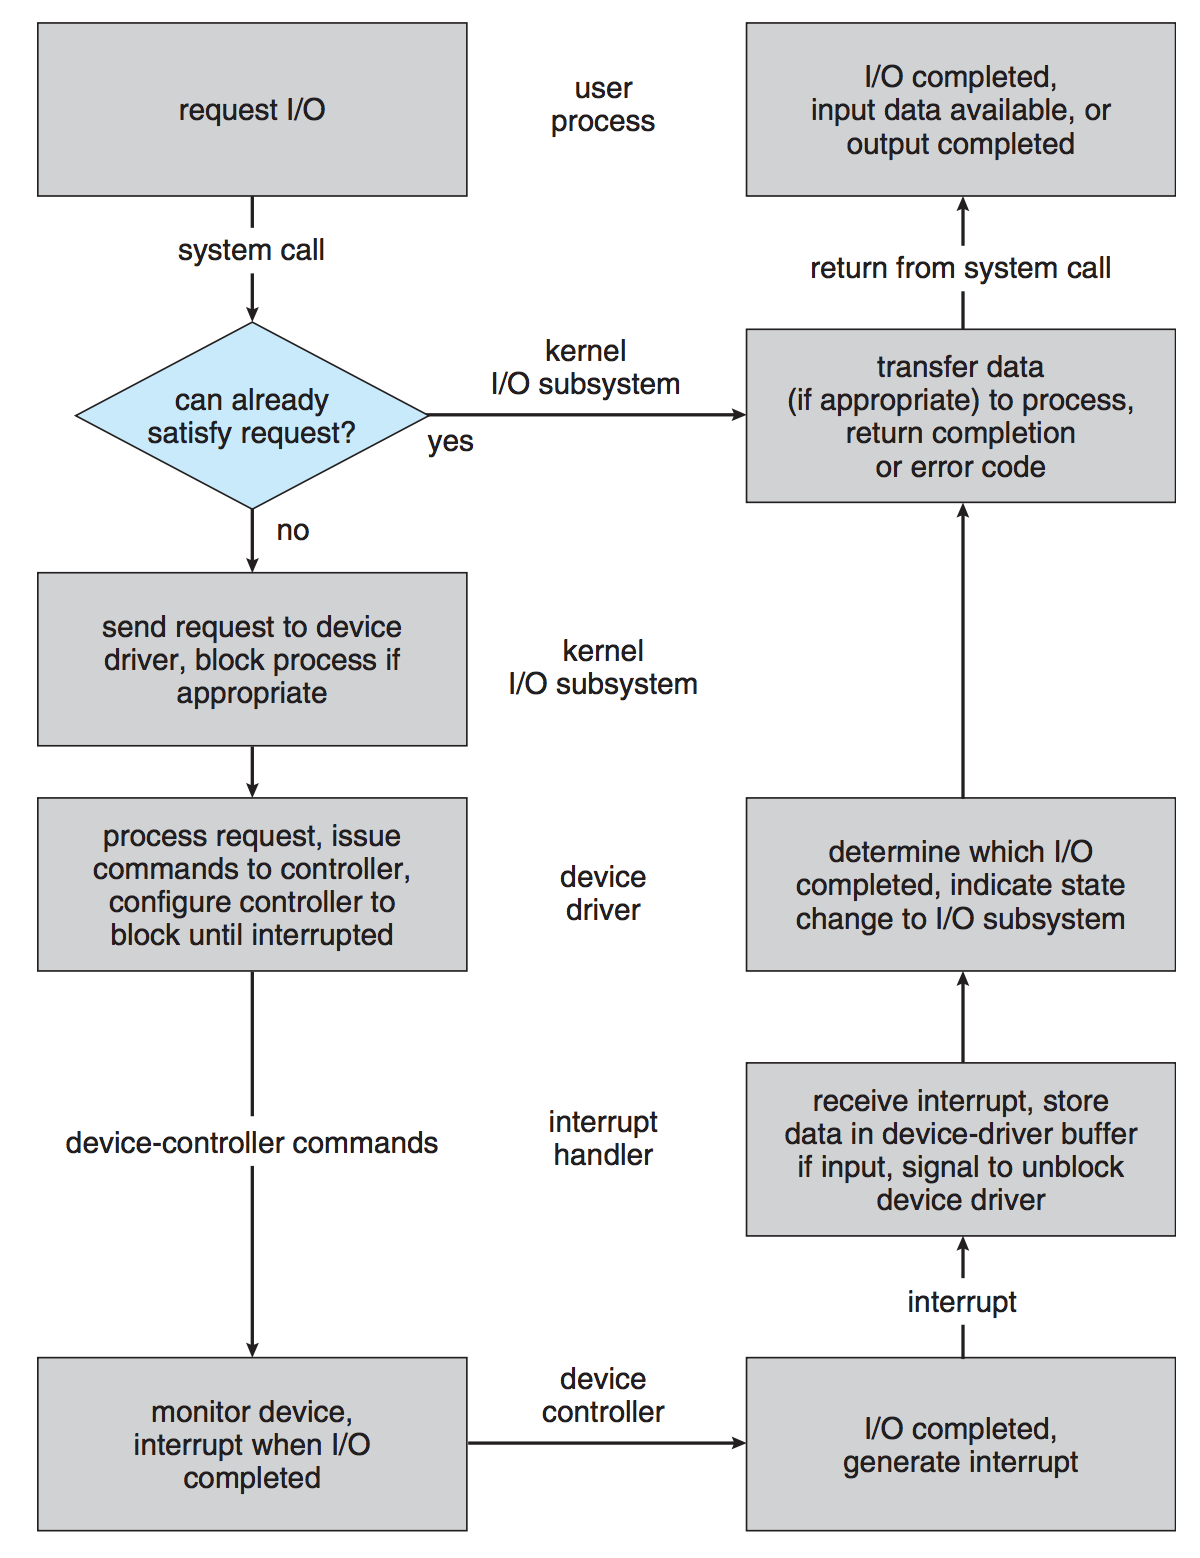
\includegraphics[width=0.65\textwidth]{images/io-lifecycle.png}\\
	The life cycle of an I/O request~\cite{osc}.
\end{center}

In general, the life cycle follows some ten steps from start to finish~\cite{osc}:

\begin{enumerate}
	\item A process issues a \texttt{read} command (assume the file is already open).
	\item The system call routine checks the parameters for correctness. If the data is in a cache or buffer, return it straight away.
	\item Otherwise, the process is blocked waiting for the device and the I/O request is scheduled. When the operation is to take place, the I/O subsystem tells the device driver.
	\item The device driver allocates a buffer to receive the data. The device is signalled to perform the I/O (usually by writing into device-control registers or sending a signal on a bus).
	\item The device controller operates the hardware to do the work.
	\item The driver may poll for status, await the interrupt when finished, or for the DMA controller to signal it is finished.
	\item The interrupt handler receives the interrupt and stores the data; it then signals the device driver to indicate the operation is done.
	\item The device driver identifies what operation has just finished, determines the status, and tells the I/O subsystem it is done.
	\item The kernel transfers the data (or error code or whatever) to the address space of the requesting process, and unblocks that process.
	\item When the scheduler chooses that process, it resumes execution.
\end{enumerate}

\bibliographystyle{alphaurl}
\bibliography{350}


\end{document}